\section{Design \label{sec:design}}
When reading both section \ref{sec:design} and section \ref{sec:implementation}, it should be acknowledged that the outline of the report represents a linear approach. This is however not how neither the prototype nor the report was written. Instead of following a linear approach, an agile approach with several iterations was used. These iteration cycles follow an iteration of the requirements, as defined in Table \ref{tab:requirements}. Each iteration includes its own minor design and implementation phase. Likewise, the iteration may change both content of the report and implementations, created in earlier iterations. The result of all these iterations leaves the final prototype.
\newline\newline
Based on the analysis, a three-part prototype is proposed. 
\begin{itemize}
    \item The first part will consist of transforming DTOs into schemas, and therefore be referred to as a \textit{Schema Provider}.
    \item The second part will consist of transforming schemas into SDKs, and be referred to as a \textit{Schema Consumer}.
    \item The third is a version difference checker, and the called \textit{Diff Checker}
\end{itemize}
The overall design of the proposed prototype can be viewed in Figure \ref{fig:mapping_flow}. 
Furthermore, the design of each part will be explored in the following sections.
\begin{figure}[h]
    \centering 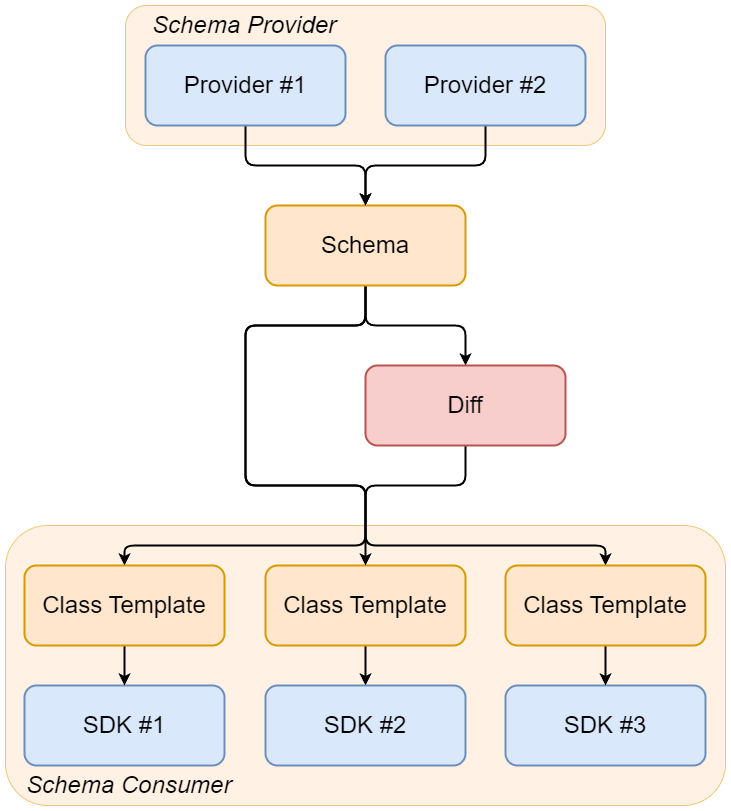
\includegraphics[height=10cm]{figures/assets/mapping_flow.png}
    \caption{Flow of entire solution}
    \label{fig:mapping_flow}
\end{figure}


\subsection{Creating a schema definition \label{sec:design:scema_definiton}}
The backbone of the entire prototype is the schema. 
DTOs will be converted into schemas, and SDKs will created from schemas.
The purpose of this schema is to define the structure of the DTO, and potentially act as the single source of truth.
While iterating over the design, the schema has changed format multiple times. 
Each of these designs will be referred to as a phase. 
Before the final schema definition is explained, the phases leading to the final definition are explained.
\begin{itemize}
    \item \textbf{Phase 1: File format}: The decision of the file format. The two proposed formats are YAML and JSON. As YAML is both more human readable, and a superset of JSON \cite{yaml_definiton}, this format was chosen, while still leaving the option for users to use JSON, if wanted.
    \item \textbf{Phase 2: List vs Map}: When defining the models, this phase went back and forth between whether the models should be in a list, with each model as an entry, or in a key-value map, with the key being the unique identifier of the object. This key would often be \( \{namespace\}.\{className\} \), however, this will not be a requirement. A key-value approach is chosen here, based on mainly two reasons; it is easier for humans to quickly see what type it is, and by taking inspiration from OpenAPI.
    \item \textbf{Phase 3: Additional properties}: When exploring hierarchy, it was identified the original definition was lacking properties necessary to implement this. To solve this, additional optional properties were added to the definition. If these properties are not needed, the schema can omit them.
    \item \textbf{Phase 4: Schema Type}: When exploring enums, it was identified that a single format for schemas is insufficient, as a class an enum is different, and thereby needs different properties. Therefore, a required property called \textit{type} was introduced, specifying if it is a class or an enum schema, and a new enum schema was created.
    \item \textbf{Phase 5: Generics}: Like in phase 3, new properties were needed when adding generics, however, this is not all that is required here. When defining a type, it is until now guaranteed to be a valid class. However, with the addition of generics, the type can now be either a generic \textit{T} or a type with a generic type, e.g. \textit{List\textless T\textgreater} or \textit{List\textless string\textgreater}. For classes, an additional optional property was added. For class properties, the same syntax as both C\#, Java, TypeScript, and other languages was used, meaning the value will be written the same as was just showcased. This means the Schema Consumer will be able to check if the type contains a \textless to indicate if it is a generic. Furthermore, it will be possible to detect if it is a class generic argument, or an implementation, by matching the type with the generic types that are defined in the class.
\end{itemize}
\noindent
By undergoing all of these phases, the final design is ready. The definition itself can viewed in Table \ref{tab:schame_exmaple_final}. For a better understanding of the definition, an example is further included in Listing \ref{code:schame_exmaple_final}. Furthermore, previous definitions are included in appendix \ref{appendix:schemas}, to showcase the design journey.
\begin{table}[H]
   \small
   \centering
   \begin{ctabularx}{\textwidth}{llX}
   
   \toprule
   \multicolumn{3}{l}{\textbf{Schema Structure}} \\
   \midrule
   \textit{Field} & \textit{Type} & \textit{Description} \\ 
   \midrule
   type & string & The type of the schema, either \textit{object} or \textit{enum} \\
   namespace & string & Which namespace the class belongs to \\
   name & string & The name of the class \\

   \midrule
   \multicolumn{3}{l}{\textbf{Object Schema Structure : Schema Structure}} \\
   \midrule
   \textit{Field} & \textit{Type} & \textit{Description} \\ 
   \midrule
   abstract? & boolean & If the class is an abstract class \\
   extends? & string & Which class the class extends \\
   generics & string[] & A list of all the generic values the class contains \\
   properties & Property[] & A list of all the properties the class contains \\

   \midrule
   \multicolumn{3}{l}{\textbf{Enum Schema Structure : Schema Structure}} \\
   \midrule
   \textit{Field} & \textit{Type} & \textit{Description} \\ 
   \midrule
   values & string[] & A list of all the enum values \\
   
   \midrule
   \multicolumn{3}{l}{\textbf{Property Structure}} \\
   \midrule
   \textit{Field} & \textit{Type} & \textit{Description} \\ 
   \midrule
   type & string & The type of the property, either a built-in type, or the key in the schema map. \\
   name & string & The name of the property \\
   nullable & boolean & If the property is marked as nullable \\
   \bottomrule
   \end{ctabularx}
   \caption{Schema definiton} 
   \label{tab:schame_exmaple_final}
\end{table}

\begin{lstlisting}[caption={Schema definition}, label={code:schame_exmaple_final}, style=yaml]
schemas:
  "SchemaExtractor.Model.Example.Person":
    type: "object"
    namespace: "SchemaExtractor.Model.Example"
    name: "Person"
    generics:
    - "T"
    properties:
    - type: "string"
      name: "Name"
      nullable: false
    - type: "SchemaExtractor.Model.Example.Gender"
      name: "Gender"
      nullable: false
    - type: "T"
      name: "GenericProp"
      nullable: true
    - type: "List<SchemaExtractor.Model.Example.Person<T>>"
      name: "Parents"
      nullable: false
    - type: "Map<string, SchemaExtractor.Model.Example.Address>"
      name: "Address"
      nullable: false
  "SchemaExtractor.Model.Example.Gender":
    type: "enum"
    namespace: "SchemaExtractor.Model.Example"
    name: "Gender"
    values:
    - "Male"
    - "Female"
  "SchemaExtractor.Model.Example.Address":
    type: "object"
    namespace: "SchemaExtractor.Model.Example"
    name: "Address"
    properties:
    - type: "string"
      name: "Street"
      nullable: false
    - type: "int32"
      name: "Number"
      nullable: false
\end{lstlisting}

\subsubsection{Adding support for native built-in types}
By deep diving into Listing \ref{code:schame_exmaple_final}, it shows some types does not define a full path, such as string and int32.
This is due to the schema having some ''\textit{built-in-types}''. These are types that are not defined as schemas, but instead a native part, which a Schema Consumer should be able to consume. Table \ref{tab:built_in_types} lists all the built-in types. If a property uses a type that is not defined here, it should be defined as its own schema.

\begin{table}[H]
   \small
   \centering
   \begin{ctabularx}{\textwidth}{lX}
   
   \toprule
   Type & Description \\
   \midrule
   boolean & A boolean input \\
   int32 & A 32-bit signed integer \\
   int64 & A 64-bit signed integer \\
   float & A 32-bit floating point \\
   double & A 64-bit floating point \\
   char & Represent a single character \\
   string & A collection of characters, as a single string. \\
   object & A wildcard type. This type has not explicitly been stated, and everything should be accepted. \\
   guid & A GUID / UUID \\
   date & A date, that includes both date and time \\
   dateOnly & A date, that only specifies the date and not the time \\
   dateTimeOffset & A date, that includes both date, time, and time offset \\
   List & A list of items. \\
   Map & A key-value pair. Often referred to as either a map or dictionary in code. \\
   \bottomrule
   \end{ctabularx}
   \caption{Built In Types} 
   \label{tab:built_in_types}
\end{table}

\subsubsection{Adding support for generics}
The adaptation of generics has a significant impact on the schema definition.
The major decision is between should the schema be updated with new fields, or should the generics be added to the current schema, and have a custom parser.
The later option is chosen, where a property type is defined the same was, as both \textit{C\#}, \textit{Java} and \textit{TypeScript}. To change e.g. a \textit{string} type, to a generic string list, the type is updated to \textit{List\textless string\textgreater}. When parsing a type, there should therefore be checked for \textit{\textless}, and if found, the type should be parsed as a generic type.
A pseudo implementation is suggested in Algorithm \ref{alog:parse_type}
\begin{algorithm}
\caption{Parse Type}
\label{alog:parse_type}
\begin{algorithmic}[1]

\Function{parseType}{type}
    \State genericStart $\gets$ indexOf(type, "\textless")
    \If{genericStart == -1}
        \State \textbf{return} type
    \EndIf

    \State splitType $\gets$ split(type, genericStart)
    \State genericType $\gets$ splitType[0]
    \State genericImpl $\gets$ parseType(substring(splitType[1], 0, length(splitType[1]) - 1))
    \State \textbf{return} combine(genericType, genericImpl)
\EndFunction
\end{algorithmic}
\end{algorithm}

\subsection{Designing a schema provider \label{sec:design:schema_provider}}
By having understood the schema, the Schema Provider can now be designed. The purpose of this is to take an existing solution and convert all DTOs defined here into schemas. This will enable the solution to act as a single source of truth for all DTOs.
It is possible to create multiple schema providers if the code base is scattered across multiple languages.
\newline\newline
The schema provider works by taking a single DTO, and from that output all necessary schemas. 
The reason why a single DTO can output multiple schemas is that both derived classes and classes used in properties should be defined. This is a recursive process, where the same steps are performed for all property types and derived types.
An example of this is showcased in Figure \ref{fig:schema_provider_flow}, where a single DTO outputs five different schemas. 
These generated schemas would be:
\begin{itemize}
    \item The own class itself
    \item The class it derives from, in this example called \textit{ParentClass}
    \item All the classes used in the properties of the class, in this example \textit{ClassOne}, \textit{ClassTwo} and \textit{ClassThree}
\end{itemize}

\begin{algorithm}
\caption{Pseudo code for converting a DTO to a schema}
\label{code:schema_provider_pseudo}
\begin{algorithmic}[1]

\State allSchemas $\gets$ []

\Function{convertClass}{type}
    \If{type is in allSchemas}
        \State \textbf{return}
    \EndIf

    \State allSchemas.add(generateSchema(type))

    \If{type.isDerived}
        \State convertClass(type.parentType)
    \EndIf

    \For{each property in type.properties}
        \State convertClass(property.type)
    \EndFor
\EndFunction

\end{algorithmic}
\end{algorithm}

\begin{figure}[h!]
    \centering
    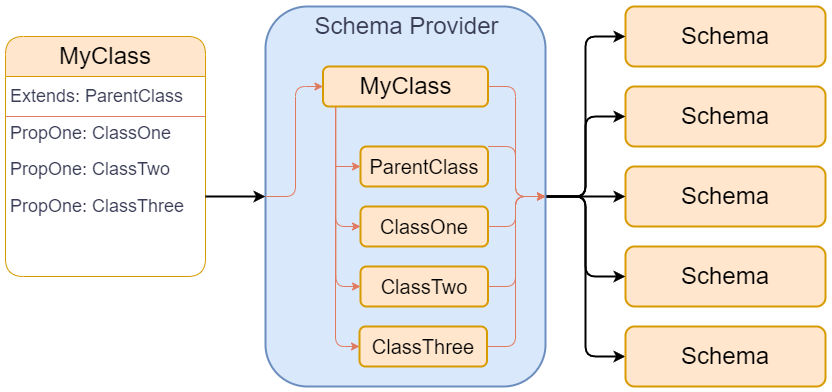
\includegraphics[width=\textwidth]{figures/assets/schema_provider_flow.png}
    \caption{Schema Provider flow}
    \label{fig:schema_provider_flow}
\end{figure}


\subsection{Designing a schema consumer \label{sec:design:schema_consumer}}
To create the final SDKs, the specified schemas should be consumed, an transformed into code.
As showcased in Figure \ref{fig:mapping_flow}, a single schema can be turned into multiple templates, and thereby into a class in an SDK.
The individual journey for creating a single SDK is illustrated in Figure \ref{fig:schema_consumer_flow}, and will be looped for each target language.

\begin{figure}[h!]
    \centering
    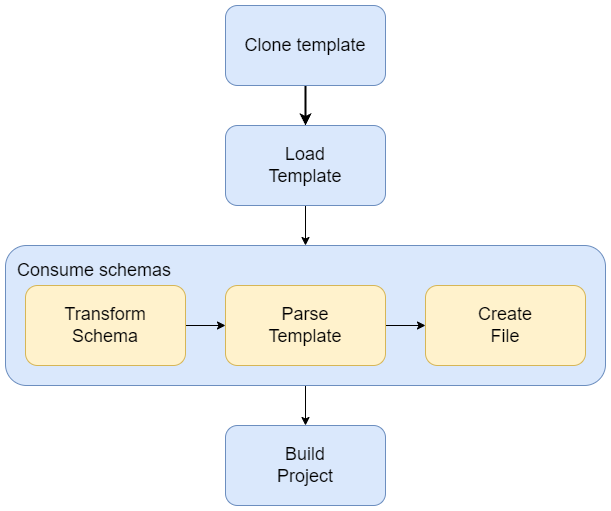
\includegraphics[width=12cm]{figures/assets/schema_consumer_flow.png}
    \caption{Schema Consumer flow}
    \label{fig:schema_consumer_flow}
\end{figure}

\noindent
Furthermore, the steps are explained in detail here.
\begin{itemize}
    \item \textbf{Clone template}: The target language template is cloned to the output. What is included in this template, will be explored in Section \ref{sec:design:default_projects}.
    \item \textbf{Load template}: The class template for the target language is loaded and parsed, allowing for quick placeholder replacement.
    \item \textbf{Consume schemas}: The following steps will be executed for each schema that should be converted.
    \begin{itemize}
        \item \textbf{Transform schema}: The schema is transformed to a language-specific data container, allowing for custom parsing of data, e.g. properties.
        \item \textbf{Parse template}: The class template is parsed with the data, resulting in a complete class.
        \item \textbf{Create file}: The class is written to a file, with a file type associated with the language.
    \end{itemize}
    \item \textbf{Build project}: The project is built, using the language-specific build tools.
\end{itemize}


\subsubsection{Adding default template projects \label{sec:design:default_projects}}
As specified, it should be possible to clone a default project, as each language has a file structure that needs to be followed. The alternative is to programmatically create files and populate these files with data, however, since the default files remain the same, they are simply cloned instead.
This means that the developer can create a template project via the language's own tools, and build the SDK on top of this. If multiple versions of the same language should be added, the developer can then simply create two templates, one with each version. Furthermore, different package managers, default dependencies, and similar things can be included in this template. This may result in a large number of default projects, but that is by design, as it can cater to everyone's specific needs.


\subsection{Designing a semantic difference checker \label{sec:design:diff_checker}}
The job of the Diff Checker is to find all semantic differences between a list of schemas.
This can be done by taking all the schemes and removing the shared schemas, as shown in equation \ref{equation:diff_set}.
\begin{equation}
\label{equation:diff_set}
    \Delta = A \bigcup B - A \bigcap B
\end{equation}
\noindent
An example of this is shown in Figure \ref{fig:diff_checker}, which shows two lists, and old list \textit{A}, and a new list \textit{B}.
\begin{figure}[h ]
    \centering
    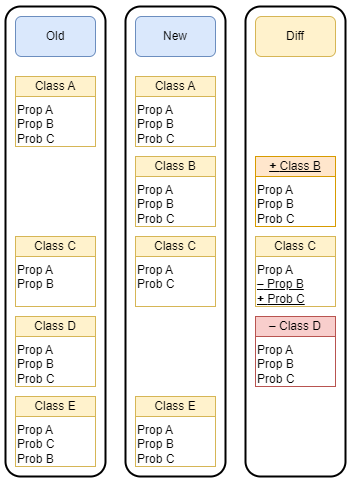
\includegraphics[height=12cm]{figures/assets/diff_checker.png}
    \caption{Diff checker result}
    \label{fig:diff_checker}
\end{figure}
\noindent
The Diff Checker will compare the figures semantically, meaning the order of properties does not matter, as long as all properties are included.
\begin{itemize}
    \item \textbf{Class A}: Two identical classes, and therefore there is no difference.
    \item \textbf{Class B}: A new class that has been added
    \item \textbf{Class C}: A class where a property has been removed, and replaced with another
    \item \textbf{Class D}: A class that has been removed
    \item \textbf{Class E}: A class where the order of properties has been switched, but remains semantically identical, which results in there being no difference.
\end{itemize}
In this case, both \textit{Class C} and \textit{Class D} should give a warning, as these classes have changed. As \textit{Class B} is a new addition, there is no need for a warning, and it can be added. From here, a developer should determine if the changes the Diff Checker warns about are acceptable or not. An acceptable change could be a planned change, where they are aware it is a breaking change. Are the changes accepted, the schemas can be transformed to an SDK, and the schemas the Diff Checker checks against can be updated with the new content.